
%(BEGIN_QUESTION)
% Copyright 2006, Tony R. Kuphaldt, released under the Creative Commons Attribution License (v 1.0)
% This means you may do almost anything with this work of mine, so long as you give me proper credit

A positive-displacement hydraulic pump may be likened to an electrical source, because it is the point of energy input into an electrical system:

$$\includegraphics[width=15.5cm]{i00761x01.eps}$$

But what kind of electrical source best mimics a positive-displacement hydraulic pump turned at a constant speed, a {\it voltage} source or a {\it current} source?

$$\includegraphics[width=15.5cm]{i00761x02.eps}$$

Also, something must be present in the electrical model to represent the compressibility of air.  What is this ``something else?''

\underbar{file i00761}
%(END_QUESTION)





%(BEGIN_ANSWER)

Positive-displacement hydraulic pumps turned at constant speed are best modeled as {\it current sources}, which is why they require pressure-relief valves to maintain constant hydraulic pressure (``voltage'').

%(END_ANSWER)





%(BEGIN_NOTES)

$$\includegraphics[width=15.5cm]{i00761x03.eps}$$

%INDEX% Mechanics, fluid power systems: positive displacement pump likened to an electrical current source

%(END_NOTES)


